% This is based on the LLNCS.DEM the demonstration file of
% the LaTeX macro package from Springer-Verlag
% for Lecture Notes in Computer Science,
% version 2.4 for LaTeX2e as of 16. April 2010
%
% See http://www.springer.com/computer/lncs/lncs+authors?SGWID=0-40209-0-0-0
% for the full guidelines.
%
\documentclass{llncs}
\usepackage{float}
\usepackage{graphicx} % Required to insert images
\usepackage{url} % To format links
\usepackage[portuguese]{babel}
\usepackage[utf8]{inputenc}

\begin{document}
\title{Redes de Computadores}
\subtitle{1º Ensaio Escrito}
%                                     also used for the TOC unless
%                                     \toctitle is used
%
\author{Paulo Caldas(a79089), Pedro Henrique(a77377), Vitor Peixoto(a79175)}
%

\institute{Universidade do Minho\\}


\maketitle              % typeset the title of the contribution

\begin{abstract}
    A humanidade carateriza-se pela constante insatisfação com os recursos que temos no presente e pela ansiedade de querer sempre mais. Devido a essa necessidade, fomos sempre evoluindo. No caso das redes móveis estamos a evoluir a um ritmo bem rápido. Neste ensaio iremos abordar a evolução de 4G para 5G, onde é que essas duas tecnologias se intersetam, onde se distinguem e um pouco da engenharia por detrás dessas redes.
    %O surgimento e evolução da tecnologia derivam de necessidades humanas. Uma das mais importantes é a comunicação e, por isto, não é surpreendente pensar que a transmissão de informação seja uma das beneficiárias de tal evolução. Inicialmente localizada, houve a necessidade de comunicar a longas distâncias, o que após vários séculos nos trouxe vários desenvolvimentos nas tecnologias de telecomunicação.%
    \keywords{Redes Computadores dados móveis 4G 5G}
\end{abstract}
%
\section{Uma breve história}
\hspace*{1.5em}A evolução das tecnologias utilizadas em transferência de dados móveis e o resultante aumento de capacidade de taxa de transferência levou à separação das várias eras por gerações que, até ao momento, são:
\subsection{1G}
%VP - Os primórdios da comunicação móvel começam na década de 80 pela Primeira Geração (1G). Esta geração usava sinais de rádio analógicos que eram transmitidos entre duas torres de rádio. Comparado às tecnologias dos seus antecessores (Geração Zero) é inferior em alguns aspetos devido ao facto de ter uma menor capacidade, handoff desconfiável e nenhuma segurança devido ao facto da chamada ser efetuada por sinais de rádio que podem ser intercetados por qualquer pessoa.%
\hspace*{1.5em}Os primórdios da comunicação móvel começam na década de 80 pelo inicial 1G, cujo G significa "geração". Esta era a primeira tecnologia de comunicação móvel, e era marcada por comunicação analógica(1) com torres de rádio, permitindo chamadas de voz entre utilizadores. Como seria de esperar pela era quando começou, esta tecnologia era aplicada em dispositivos de comunicação com menos funcionalidades que as dos dias de hoje, entre as quais "pagers" e telefones sem fios \cite{Ton:Pan:Kus}
\subsection{2G}
\hspace*{1.5em}A segunda geração que foi introduzida no fim da década de 80 \cite{Ton:Pan:Kus} foi marcada pela era digital. As chamadas continuavam a ser enviadas via rádio, mas foi introduzida a prática de codificação digital. Ou seja, a informação que era transmitida pelos dispositivos móveis era inicialmente codificada digitalmente, e isto garantia várias vantagens entre as quais a diminuição de ruído e diminuição de consumo de bateria comparando com a antiga geração analógica.
\subsection{3G}
\hspace*{1.5em}Esta geração foi inicialmente disponibilizada no inicio do século 21. Esta foi marcada por uma maior taxa de transferência de informação que consequentemente disponibilizou um conjunto de aplicações que antes seriam impossíveis, entre as quais:
\begin{itemize}
    \item GPS
    \item Televisão
    \item Conferências de vídeo
\end{itemize}
\subsection{4G}
4G
\hspace*{1.5em}A geração mais atual com uso em massa é a quarta, e é marcada com um conjunto de especificações que superiorizam as capacidades da geração anterior. Apesar de bastantes empresas publicitarem os seus serviços como 4G, bastantes deles não cumprem toda a gama de padrões definidos pela ITMA (International Mobile Telecommunications Advanced), entre as quais(5):
\begin{itemize}
    \item Deve ser baseada num "IP packet switching" contra a alternativa de "circuit switching".
    \item Taxas de transferência de informação de 100Mb/s numa rede com bastante movimento, e de 1Gb/s em regiões de acesso "wireless" local.
\end{itemize}
\section{A passagem para 5G}
\hspace*{1.5em}O aparecimento de uma nova geração advém do crescimento constante da necessidade de serviços móveis. Isto poderá dever-se a ambos o crescimento do número de "smartphones" ativos globalmente, bem como a proliferação do conceito de "internet of things", em que cada vez mais existem os mais varados tipos de sistemas embebidos que nos rodeiam (desde frigoríficos a aspiradores) que necessitam de uma ligação de dados móveis. De facto, está previsto o tráfego de dados móveis aumentar entre 20 a 50 vezes nos próximos 5 anos e em 2019 estima-se que esse tráfego aumente cerca de 24,3 exabytes (24,3 milhões de terabytes) por mês. \cite{Fei} Com efeito, é praticamente impossível para as tecnologias das redes 3G e 4G acompanhar este ritmo de crescimento. Para corresponder a este ritmo, a humanidade tem trilhado um caminho para o nascimento da 5ª geração de redes móveis.
\\
\hspace*{1.5em}A rede LTE (4G) é ainda a geração de rede móvel mais usada em todo um mundo, com cerca de 69\% do tráfego móvel a ser efetuado por essa tecnologia \cite{cisco}. Esta rede é caraterizada pela mudança de uma tecnologia de informação híbrida (dados+voz) da rede 3G para uma rede IP de dados apenas.
Por outro lado o 5G eleva a fasquia da tecnologia permitindo uma matriz de MIMO 16x16 até 256x256. \\
A teclonogia 5G promente, entre outros objectivos:
\begin{itemize}
    \item Capacidade 1000 vezes maior
    \item Velocidade 10Gbits/s
    \item Latências menores que 1ms
\end{itemize}
Seguem-se um conjunto de conceitos de comunicação móvel que necessitam de ser melhorados a modo de cumprir os requisitos prometidos pela tecnologia 5G. \\
% PH
\section{Desafios para a nova geração}

\subsection{Mobilidade e manutenção}
% PH - Verificar correção científica da descrição das estação de base que pode desbloquear questão na intro. (sinais rádio == sinais eletromagnéticos?) %
\hspace*{1.5em}Mobilidade de informação é um dos desafios relativamente a comunicações entre dispositivos móveis. Para tal, é necessário definir infraestruturas e modos de comunicação rápidos e fiáveis. Um equipamento necessário é chamado de estação de base: torres de telecomunicações rádio que, servindo-se de antenas, agem como transmissores e recetores de sinais rádio e cooperam com aparelhos móveis na tarefa de distribuição de informação entre si.
Uma alternativa inicial passava por construir uma torre grande com bastante alcance, cobrindo uma grande área. As principais desvantagens deste sistema passam por:
\begin{itemize}
    \item Torre necessita de ter muita potência, pelo que a sua manutenção é geralmente mais complicada;
    \item Criam um sistema pouco robusto: a avaria de uma torre implica que uma vasta região fique sem sinal.
\end{itemize}

\hspace*{1.5em}A solução atual para estas desvantagens passa por ao invés de utilizar uma torre com bastante potência, substituí-la por uma rede de torres com menores potências. Disto resulta:

\begin{itemize}
    \item Possibilidade de cobrir várias regiões que normalmente seriam impossíveis de alcançar
    \item Maior robustez: uma torre pode entrar em manutenção sem comprometer a integridade de toda a rede
    \item Reutilização de frequências: várias torres espalhadas geograficamente permite que a mesma frequência seja utilizada em regiões diferentes
\end{itemize}

\begin{figure}[H]
    \centering
    \begin{minipage}{0.45\textwidth}
        \centering
        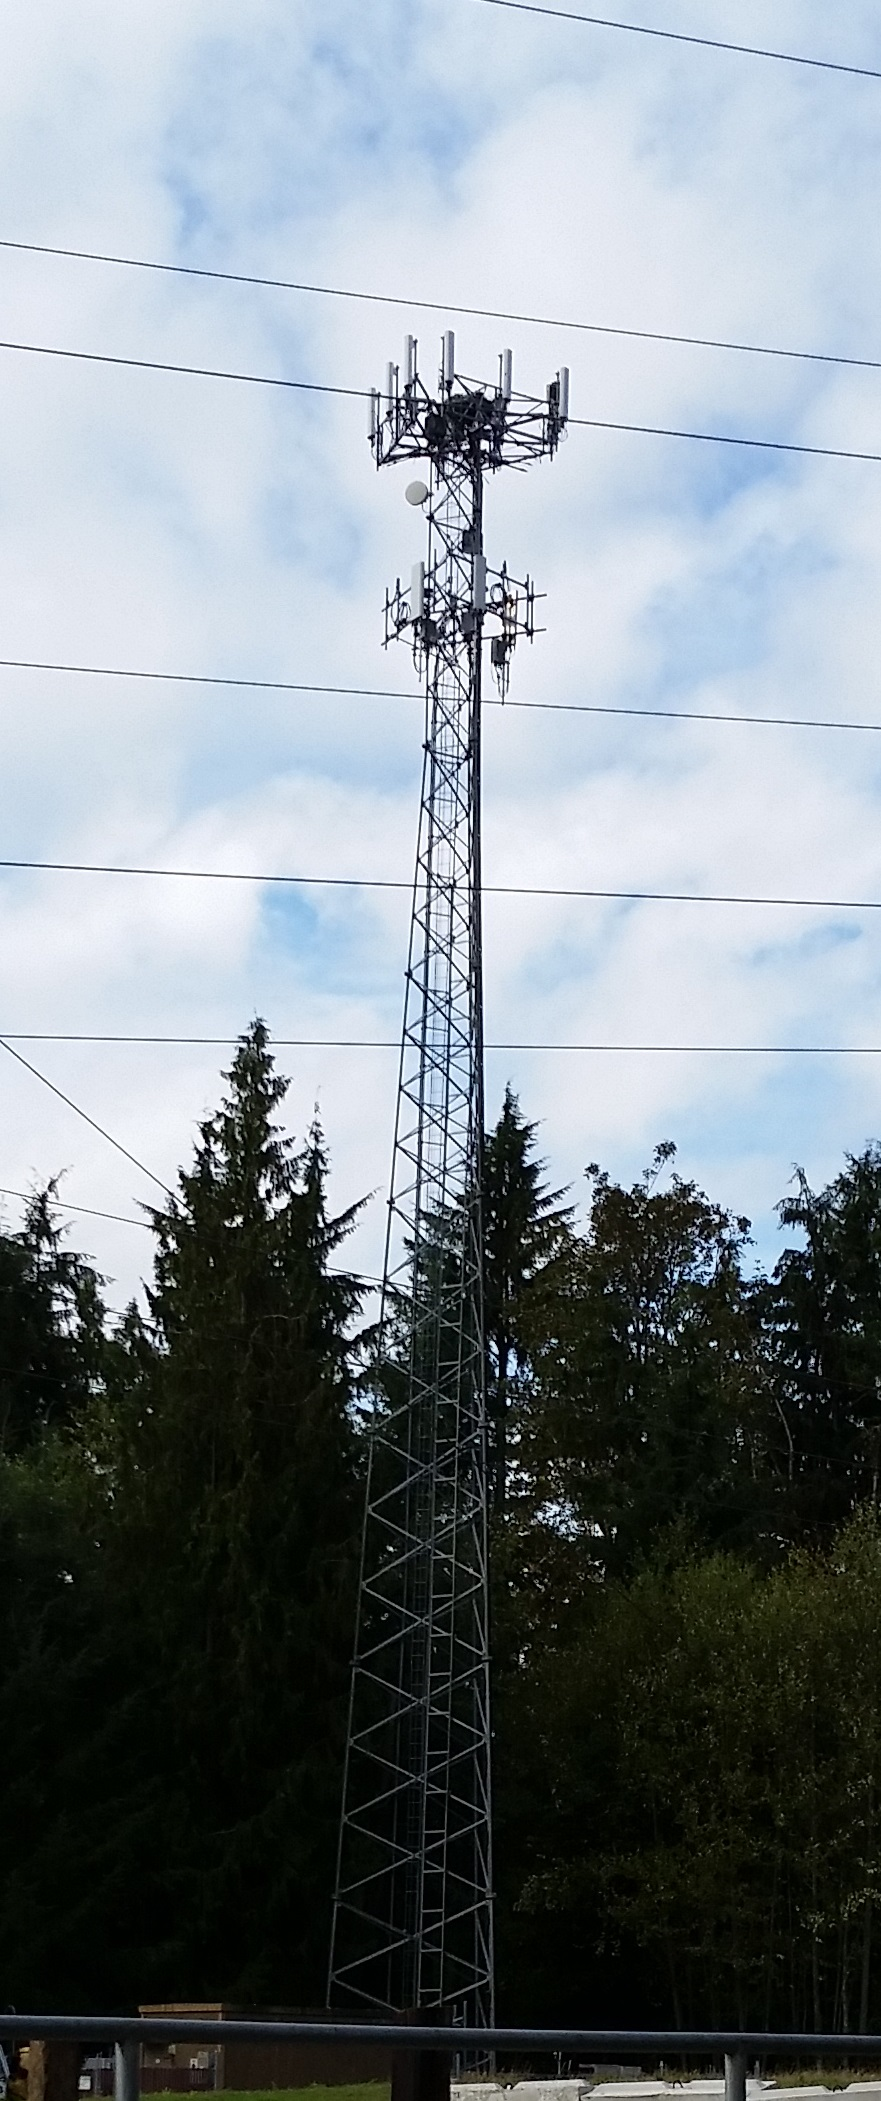
\includegraphics[scale = 0.128]{torre.jpeg}
        \caption{Torre rádio \cite{img1}}
    \end{minipage}\hfill
    \begin{minipage}{0.45\textwidth}
        \centering
        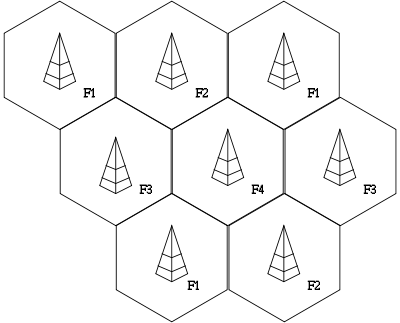
\includegraphics[scale=0.5]{network.png}
        \caption{Redes de torres móveis \cite{img2}}
    \end{minipage}
\end{figure}

\section{Áreas para melhoria}

\subsection{Latência}

A minimização do período de latência é essencial para usos atuais que exigem algum tipo de comunicação em tempo real como conferências de vídeo e voz \textit{over IP}, aplicações com funcionalidades de cooperação em simultâneo, sincronização de ficheiros e de serviços de email, jogos, entre outros.

A latência poderá ser dividida em :
\begin{itemize}
	\item \textit{\textbf{User plane latency}}, também conhecida como \textit{round-trip time} (RTT), que consiste no período de tempo que leva a um pacote partir do equipamento fonte e chegar ao destino em adição ao tempo que leva a fazer o caminho inverso. Exclui o tempo de processamento do pacote no destino;
	\item \textit{\textbf{Control plane latency}}, que consiste no tempo que um dispositivo leva a passar do estado \textit{RRC idle} para o estado \textit{RRC connected} e assim tornar-se capaz de transferir dados.
\end{itemize}

A latência poderá diminuir com avanços que afetem não só a \textit{user plane latency} e a \textit{control plane latency}, mas também a arquitetura da \textit{core network}. Com base na referência [1], o requerimento da tecnologia 4G LTE para as latências nos \textit{user plane} e \textit{control plane} são de 20 e 100 ms, enquanto que os valores que a 5G toma como alvo são de 1 ms e de 10 ms, respetivamente. No caso de estudo, apenas um dos operadores conseguiu valores médios (80 ms) de \textit{control plane latency} abaixo do requerimento, pelo que se espera que nas implementações comerciais de tecnologias 5G os requerimentos sejam cumpridos, de modo a possibilitar os vários usos para os quais a mínima latência é crítica.

Possíveis soluções passariam por :
\begin{itemize}
	\item \textit{\textbf{network slicing}}, que permite criar redes lógicas sobre a infraestrutura físicas e assim torná-la mais dinâmica e adaptável a diferentes usos. Os recursos, como espaço de armazenamento, nodos de transporte e processamento, podem ser dedicados a uma \textit{slice} ou partilhados entre diferentes \textit{slices}. Uma \textit{network slice} é criada para satisfazer um comportamento que se deseja de uma rede. Esse comportamento pode estar associado a segurança, isolamento do fluxo de dados, qualidade de serviço, fiabilidade, entre outros;
	\item \textit{\textbf{edge computing}}, que apostando na descentralização dos dados e do seu processamento, permitiria que estes se encontrassem mais próximos dos limites da rede (mais próximos dos utilizadores e seus equipamentos) e assim diminuir a latência.
\end{itemize}

\subsection{Handover}

O \textit{handover} corresponde ao processo de transferência de uma ligação entre canais ligados a uma \textit{core network}. É um processo essencial na gestão e garantia da mobilidade de equipamentos e respetivos utilizadores pelo espaço abrangido por redes celulares. Estas comutações podem ocorrer quando um equipamento se está a afastar em demasia de uma estação-base original e a aproximar-se de uma outra, entrando na sua área de abrangência, e assim evitar perda de ligação devido à atenuação do sinal, ligando-se à nova estação-base; ou quando se esgota a capacidade para novas conexões a uma estação-base, e nesse caso, estando o utilizador numa zona de sobreposição com a zona de abrangência (célula) de uma outra, se dá a ligação a essa outra estação-base, entre outras razões.

O \textit{handover} pode ser de 2 tipos :
\begin{itemize}
	\item \textbf{hard \textit{handover}} (ou break-before-make), é implementação escolhida pela tecnologia 4G LTE e consiste na quebra da ligação ativa com uma estação-base, de modo a que o dispositivo se ligue a outra, estando na sua área de alcance. Este método obriga então a um período em que a ligação deixa de existir, entre o momento em que o dispositivo do utilizador se desliga da estação-base original e se liga à nova. No caso da referência [1], na zona onde foram efetuados os testes, o tempo medido de inatividade no handover apresentava uma mediana na ordem dos 40 ms. Este tempo revela-se desadequado e impossibilita vários dos planos de uso pretendidos para implementações de tecnologias 5G, tais como meios de transporte autónomos e \textit{platooning}, onde o conhecimento da localização e velocidade dos veículos a cada momento é fulcral. Para além disto, verificou-se que a ligação se perdia em 1\% dos \textit{handovers} tentados. O subsequente processo de restabelecimento da ligação aumenta a duração do \textit{handover} para vários segundos, o que, novamente, impossibilita o sucesso de casos de uso que exijam total segurança e cuja fiabilidade e eficiência é crítica.
	\item \textbf{soft \textit{handover}} (ou make-before-break) será uma das soluções propostas para implementação na 5ª geração de redes móveis. Neste método, o equipamento conecta-se à estação-base alvo antes de se desconectar da estação-base que o serve. Prevê-se que na 5G sejam possíveis várias ligações a estações-base em simultâneo. Este plano tem custos associados devido à maior complexidade exigida aos dispositivos dos utilizadores, uma vez que necessitarão de processar vários sinais em simultâneo, e a uma maior carga sobre a rede, já que vários canais de várias estações-base estarão dedicados a uma só ligação. Em comparação, o \textit{hard handover} é mais simples, o que também se traduz em benefícios económicos, e como haverá apenas um canal ocupado por uma ligação a cada momento, a rede não se encontrará tão carregada. No entanto, a fiabilidade oferecida pelo \textit{soft handover} é significativamente maior, não apenas, mas também em situações de handover, uma vez que havendo várias ligações síncronas, o melhor sinal pode ser usado ou até poderão ser combinados os sinais de modo a obter uma melhor cópia do sinal. A complexidade adicional e maior carga sobre a rede, se ultrapassadas ou balanceadas de modo a poder usufruir dos benefícios do \textit{soft handover} sem grandes custos, abrirão portas aos usos que tanto requerem confiança nas ligações.
\end{itemize}
	
Para além desta última, na 5G prevê-se o uso de \textit{handover} sincronizado, que consiste no processo sem \textit{random access} em que o equipamento do utilizador e a estação-base, em sincronização, definem o momento em que o \textit{handover} deve ocorrer, o que constitui uma técnica benéfica em processos de handover.

\section{Casos de uso}

À medida que se registam avanços nas tecnologias, estes também se traduzem em novos casos de uso e destes existem vários que se esperam que sejam possibilitados pelas tecnologias associadas à implementação de redes móveis de 5ª geração.

Novos casos de uso que se esperam incluem :
\begin{itemize}
	\item Objetos associados à \textit{Internet of Things}, como os já existentes frigoríficos, termostatos, \textit{wearables} como \textit{smartwatches} e óculos de realidade aumentada;
	\item Aplicações na indústria como unidades industriais autónomas cujos meios de produção se podem controlar remotamente e comunicar entre si, o que traz também a melhor possibilidade de distribuição de energia. O uso de sensores conectados à rede na agricultura pode trazer também melhor eficiência no processo de irrigação e melhor controlo da qualidade das plantações;
	\item Sistemas de transporte autónomos, incluindo transportes públicos e privados, como redes ferroviárias e metropolitanas de comboios sincronizados pela rede, carros que usufruem de condução autónoma, maior eficiência no transporte de bens com recurso ao \textit{platooning}, a possibilidade de \textit{tracking} de produtos em tempo real, entre outros.
\end{itemize}

\subsection{Largura de banda}
\hspace*{1.5em} No mundo de hoje em que cada vez existem mais dispositivos móveis e que cada vez requerem maior taxa de transferência de dados. O problema é que todos estes dados são transmitidos na mesma banda, havendo uma competição por recursos que causa serviços geralmente mais lentos e queda de conexões. Uma solução passa pelo uso de sinais de espetro que normalmente não são usados, e a aplicação disso passa pelo uso de ondas milimetricas que desbloqueiam maiores larguras de banda e maiores taxas de transferência e dados \cite{Mis:El} \\
\hspace*{1.5em} Uma desvantagem, porém, é o facto de que sinais com estes comprimentos de onda criam uma dificuldade em penetrar locais físicos, como edifícios ou quaisquer obstáculos urbanos \cite{everything:to:know}, mas considerando o preço de construção e manutenção destes é necessária uma visão estratégica e económica de cada problema em questão.
\subsection{Capacidade de comunicação}
\hspace*{1.5em} Uma outra preocupação é a de aumentar a capacidade das redes de comunicação móvel. Será explorada a ideia de MIMO (multiple-input multiple-output) e mais importantemente massive MIMO, que é a aplicação de várias antenas na mesma estação com visto a aumentar a capacidade das redes móveis 22 ou mais vezes \cite{everything:to:know} e neutralizar as desvantagens do uso de ondas milimetricas. \cite{Mis:El}

\begin{figure}
    \centering
    \includegraphics[scale = 0.05]{mimo.png}
    \caption{Aplicação MIMO \cite{MIMO}}
\end{figure}

\hspace*{1.5em} Um problema que surge desta tecnologia é a ocorrência de interferência entre ondas, visto que vários transmissores estão compactados juntamente. Para tentar resolver este problema surge o conceito de "beamforming" que cria uma nova perspetiva no envio de sinais: em vez de enviar o sinal para todas as direções em volta do transmissor, tecnologias que implementem "beamforming" permitem envio de sinal apenas para o seu destino, reduzindo interferências entre ondas.
\section{Casos de uso para 5G}

%
% ---- Bibliography ----
%
\begin{thebibliography}{11}

    \bibitem{magazine} Mads Lauridsen, Lucas Chavarría Giménez, Ignacio Rodriguez, Troels B. Sørensen, and Preben Mogensen, From LTE to 5G for Connected Mobility, IEEE Communications Magazine • Março de 2017, páginas 156-162

    \bibitem{magazine2} Boyd Bangerter, Shilpa Talwar, Reza Arefi, and Ken Stewart, Intel, Networks and Devices for the 5G Era, IEEE Communications Magazine • Fevereiro de 2014, páginas 90-96

    \bibitem{website} Gustav Wikström, Daniel Larsson, LTE latency reductions: preparing for 5G, Ericsson Research Blog em \url{https://www.ericsson.com/research-blog/lte-latency-reductions-preparing-5g/}, 20 de Setembro de 2016

    \bibitem{website2} Per Synnergren, Torsten Dudda, LTE Latency Improvement Gains, Ericsson Research Blog \url{https://www.ericsson.com/research-blog/lte-latency-improvement-gains/}, 4 de Novembro de 2014

    \bibitem{website3} Osman N. C. Yilmaz, Niklas A. Johansson, 5G Radio Access for Ultra-Reliable and Low-Latency Communications, Ericsson Research Blog em \url{https://www.ericsson.com/research-blog/5g-radio-access-for-ultra-reliable-and-low-latency-communications/}, 11 de Maio de 2015

    \bibitem{whitepaper} Ericsson White Paper, 5G systems - Enabling the Transformation of Industry and Society, Janeiro de 2017

    \bibitem{Ton:Pan:Kus}
    Tondare S M,Panchal S D,Kushnure D T,
    2278-1021
    Evolutionary steps from 1G to 4.5G,
    International Journal of Advanced Research in Computer and Communication Engineering Vol. 3
    • Abril de 2014, página 1

    \bibitem{Fei}
    Fei H.,
    Opportunities in 5G Networks: A Research and Development Perspective
    • 5 de Abril de 2016, página 34

    \bibitem{everything:to:know}
    Amy Nordrum, Kristen Clark e IEEE Spectrum Staff,
    Everything You Need to Know About 5G
    • 27 de Janeiro 2017

    \bibitem{Mis:El}
    H. M. El Misilmani and A. M. El-Hajj,
    978-1-5386-3250-5/17
    Massive MIMO Design for 5G Networks: An Overview on Alternative Antenna Configurations and Channel Model Challenges,
    2017 International Conference on High Performance Computing \& Simulation
    • 17-21 de Julho de 2017, página 288
    \bibitem{img1}
    em \url{https://en.wikipedia.org/wiki/Cell_site}

    \bibitem{img2}
    em \url{https://en.wikipedia.org/wiki/Cellular_network}

    \bibitem{Android}
    Majeed Ahmad,
    4g and 5g wireless : How they are alike and how they differ
    em \url{http://www.androidauthority.com/4g-and-5g-wireless-how-they-are-alike\\
    -and-how-they-differ-615709/}
    • 24 de Setembro de 2017

    \bibitem{MIMO}
    em \url{https://www.theengineer.co.uk/uk-trials-of-massive-mimo-bring-5g-\\communications-closer-to-reality/}

    \bibitem{cisco}
    em \url{https://www.cisco.com/c/en/us/solutions/collateral/service-provider/visual-networking-index-vni/mobile-white-paper-c11-520862.html}
    • 24 de Setembro de 2017
\end{thebibliography}


\end{document}
